\documentclass[brudnopis]{xmgr}
% Jeśli nowe rozdziały mają się zaczynać na stronach nieparzystych:
%\documentclass[openright]{xmgr}

% install minted package to highlight source code
% \usepackage{minted}

%\defaultfontfeatures{Scale=MatchLowercase}
%\setmainfont[Numbers=OldStyle,Ligatures=TeX]{Minion Pro}
%\setsansfont[Numbers=OldStyle,Ligatures=TeX]{Myriad Pro}
% for fontspec version < 2.0
% \setmainfont[Numbers=OldStyle,Mapping=tex-text]{Minion Pro}
% \setsansfont[Numbers=OldStyle,Mapping=tex-text]{Myriad Pro}
%\setmonofont[Scale=0.75]{Monaco}

% Opcjonalnie identyfikator dokumentu
% drukowany tylko z włączoną opcją 'brudnopis':
\wersja   {wersja wstępna [\ymdtoday]}

\author   {Adam Makiewicz}
\nralbumu {235281}
\email    {adammak23@gmail.com}


\title    {Generowanie płytek obwodu drukowanego w środowisku Python jako dodatek do programu graficznego Blender}
\date     {2020}
\miejsce  {Gdańsk}

\opiekun  {dr P. Arłukowicz}

% dodatkowe polecenia
%\renewcommand{\filename}[1]{\texttt{#1}}
%\definecolor{stress}{cmyk}{0,1,0.13,0} % RubineRed
%\definecolor{topic}{cmyk}{0.98,0.13,0,0.43} % MidnightBlue

\begin{document}

% streszczenie
\begin{abstract}
Istnieje wiele programów do projektowania płytek drukowanych, jednak żadne z nich, z uwagi na swoje ścisłe zastosowania, nie posiadają odpowiednich narzędzi do zaawansowanego renderowania, animacji i tworzenia szeroko pojętej “sztuki”. Popularny program do tworzenia grafiki 3D - Blender, z uwagi na możliwość rozbudowania go o dodatki jest znakomitym narzędziem mogącym wspomagać ten proces.
\end{abstract}

% słowa kluczowe
\keywords{wizualizacja, grafika, 3D, Blender, Python, PCB}

% tytuł i spis treści
\maketitle

% wstęp
\introduction

Obwody drukowane czy też inaczej płytki drukowane (zwane dalej "PCB", ang. Printed Circuit Board) to podstawa dla każdego modułu elektronicznego. Dzięki swojej budowie oraz dobranym częściom składowym pozwalają inżynierom z roku na rok konstruować coraz to nowocześniejsze i bardziej funkcjonalne urządzenia. PCB służy przede wszystkim do montowania wszelkich podzespołów elektronicznych oraz zapewnienia im wspólnego stabilnego połączenia.

Tworzenie PCB składa się z trzech głównych etapów \cite{Abboud}: 

\begin{itemize}
\item
Logic Design - Stworzenie schematu logiki i reguł projektowych, spis użytych komponentów i ich wzajemnych połączeń
\item
Layout - Zaprojektowanie układu, który decyduje o fizycznym położeniu i połączeniach (tzw.  \emph{routing}) komponentów
\item
Produkcja przemysłowa
\end{itemize}
    
    Najważniejszym punktem projektowania układu jest rozmieszczenie komponentów. Ten proces jest satysfakcjonującym twórczym przedsięwzięciem i prawdopodobnie jednym z najtrudniejszych aspektów procesu projektowania PCB. Wielu inżynierów uważa go za formę sztuki gdyż w przeciwieństwie do schematu, który opiera się tylko na matematyce, jest nieco bardziej płynny i elastyczny. 

\begin{figure}[!tbh]
\centering
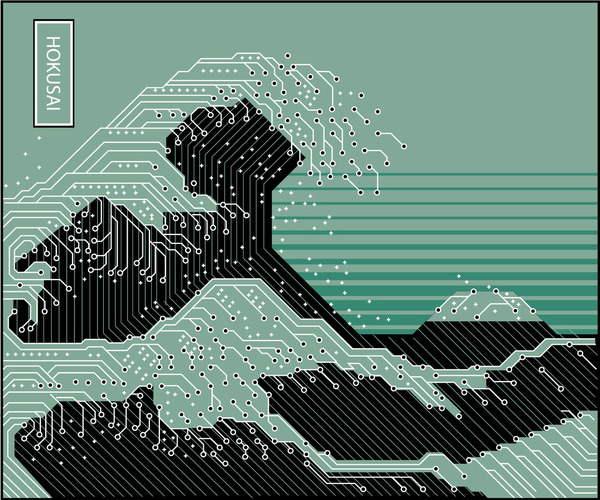
\includegraphics[width=1\hsize]{fig/hokusai}
\caption{Joel Betancourt znany jako Garabating - "Katsushika Hokusai Electronic Circuit Board"\label{RYS.2}}
\source{https://garabating.com/post/44549621917/katsushika-hokusai-electronic-circuit-board}
\end{figure}

Nie oznacza to jednak pełnej dowolności w projekcie, gdyż należy wziąć pod uwagę mnogość technicznej wiedzy, pomiarów i zależności takich jak optymalizacja długości ścieżek, ograniczenia mechaniczne i montażowe, itd.\footnote{https://www.autodesk.com/products/eagle/blog/top-10-pcb-component-placement-tips-pcb-beginner/} Z uwagi na ilość i różnorodność ograniczeń nie jest możliwa całkowita automatyzacja sprawdzania poprawności wykonanego projektu, zatem przydatna dla projektanta okazuje się wizualizacja efektu końcowego. Jest ona także niezbędnym elementem procesu marketingowego, logistycznego czy edukacyjnego. Istnieje wiele programów do projektowania PCB jednak żadne z nich, z uwagi na swoje ścisłe zastosowania, nie posiadają odpowiednich narzędzi do zaawansowanego renderowania, animacji i tworzenia szeroko pojętej “sztuki”. Popularny program do tworzenia grafiki 3D - Blender, z uwagi na możliwość rozbudowania go o dodatki jest znakomitym narzędziem mogącym wspomagać ten proces.





% ROZDZIAŁ 1


\chapter{Cel i zakres pracy magisterskiej}

Celem niniejszej pracy jest stworzenie łatwego do rozbudowania i spójnego systemu umożliwiającego import plików projektowych używanych bezpośrednio w przemyśle PCB do programu Blender, następnie interpretację i wyświetlenie pełnowymiarowego modelu 3D płytki drukowanej która powstałaby w procesie produkcji przemysłowej.

\section{Wymagania funkcjonalne}


\chapter{Opis technologii wykorzystanych w pracy}
\section{python + blender python (to, że nie da się pipa i trzeba dołączyć moduł gerber etc)}
\section{moduły zewnętrzne pythona: cairo, wheel, gerber etc.}
\section{opis plików projektowych PCB (gerber, excellon, placement, etc.)}
\section{developing w VS code? fajny linker kopiujący etc?}


\chapter{Architektura zrealizowanego systemu}
\section{Koncepcyjna struktura/podział na moduły/wzorzec projektowy?/przegląd funkcjonalności}


\chapter{Szczegóły implementacyjne systemu}
\section{Podstawowe komponenty}
\section{Funkcjonalność panelu}

\chapter{Podsumowanie}
\section{Realizacja założonych celów pracy magisterskiej}
\section {Problemy napotkane podczas realizacji systemu}
\section{Możliwości rozwoju systemu}
\section{Wnioski?}



\begin{table}[!htb]
\begin{tabular}{|l|l|l|} \hline
Nazwa & Autor      & Adres URL \\ \hline
\texttt{sablotron} & Ginger Alliance & \url{http://www.gingerall.com} \\ \hline
\texttt{Xt}        & J.~Clark & \url{http://www.jclark.com} \\ \hline
\texttt{4XSLT}     & FourThought & \url{http://www.fourthought.com} \\ \hline
\texttt{Saxon}     & Michael Kay &  \url{http://users.iclway.co.uk/mhkay/saxon} \\ \hline
\texttt{Xalan}     & Apache XML Project & \url{http://xml.apache.org} \\ \hline
\end{tabular}
\caption{Publicznie dostępne procesory XLST\label{zest:proces:xslt}}
\source{Opracowanie własne}
\end{table}


% zakończenie
\summary
Możliwości, jakie stoją przed archiwum prac magisterskich opartych na
XML-u, są ograniczone jedynie czasem, jaki należy poświęcić na pełną
implementację systemu. Nie ma przeszkód technologicznych do stworzenia
co najmniej równie doskonałego repozytorium, jak ma to miejsce w
przypadku ETD. Jeżeli chcemy w pełni uczestniczyć w rozwoju nowej ery
informacji, musimy szczególną uwagę przykładać do odpowiedniej
klasyfikacji i archiwizacji danych. Sądzę, że język XML znacznie to
upraszcza.

% załączniki (opcjonalnie):
%\appendix
%\chapter{Tytuł załącznika 1}
%Treść załącznika 1.


% literatura (obowiązkowo):
\bibliographystyle{unsrt}
\bibliography{literatura}

% spis tabel (jeżeli jest potrzebny):
\listoftables

% spis rysunków (jeżeli jest potrzebny):
\listoffigures

\oswiadczenie

\end{document}
